%%
%% FINAL REVISION — Cascaded Semantic Deduplication with Adaptive Information Budgeting
%% All numbers from real data. Placeholders marked with %%PLACEHOLDER for pending experiments.
%% Title changed per reviewer feedback. Hamiltonian framing retained as component name, not paper identity.
%%

\documentclass[sigconf,nonacm]{acmart}

%% -------------------------------------------------------
%% Required packages
%% -------------------------------------------------------
\usepackage{booktabs}
\usepackage{float}
\usepackage{graphicx}
\usepackage{amsmath}
\usepackage{amssymb}
\usepackage{microtype}
\usepackage{pifont}
\usepackage{xcolor}
\usepackage{tikz}
\usetikzlibrary{positioning, shapes.geometric, shapes.symbols, shadows, arrows.meta, fit}

\newcommand{\cmark}{\ding{51}}%
\newcommand{\xmark}{\ding{55}}%

%% -------------------------------------------------------
%% Conference metadata
%% -------------------------------------------------------
\setcopyright{rightsretained}
\acmDOI{XXXXXXX.XXXXXXX}
\acmConference[MM '26]{ACM Multimedia 2026}{October 2026}{TBD}
\acmYear{2026}
\acmISBN{XXX-X-XXXX-XXXX-X/26/10}
\copyrightyear{2026}

%% -------------------------------------------------------
\begin{document}

\title[AdaFrame: Adaptive Video Ad Analysis]{AdaFrame: Hierarchical Multimodal Deduplication with Adaptive Information Budgeting for Cost-Efficient Video Advertisement Analysis}

\author{Abdul Basit Tonmoy}
\affiliation{%
  \institution{Wabash College}
  \city{Crawfordsville}
  \state{IN}
  \country{USA}
}
\email{atonmoy27@wabash.edu}

%% -------------------------------------------------------
\begin{abstract}
Video advertisement analysis using Vision-Language Models (VLMs) faces a critical efficiency bottleneck: uniform frame sampling wastes the majority of inference budget on redundant content, while existing keyframe methods optimize for human viewing rather than machine extraction fidelity. We propose \textbf{AdaFrame}, a three-tier hierarchical deduplication cascade---perceptual hashing, learned perceptual similarity (LPIPS), and semantic embedding clustering (CLIP)---that progressively filters redundant frames before VLM inference. Unlike fixed-rate sampling, frame budgets are determined adaptively via Intrinsic Semantic Dimensionality, which estimates each video's effective semantic complexity through SVD of frame embeddings. Evaluated against seven baselines on 484 video advertisements from the Pitt Ads Dataset, AdaFrame halves frame count and VLM cost compared to industry-standard uniform sampling with no statistically significant accuracy loss (93.7\% pairwise topic agreement; McNemar's test not significant). The cascade reduces expensive CLIP compute by 40\% through cheap perceptual pre-filtering, while temporal-aware selection adds 2.8 percentage points of accuracy over standalone clustering. Code and evaluation protocols will be released upon publication.
\end{abstract}

%% -------------------------------------------------------
\begin{CCSXML}
<ccs2012>
  <concept>
    <concept_id>10010147.10010178.10010224</concept_id>
    <concept_desc>Computing methodologies~Computer vision</concept_desc>
    <concept_significance>500</concept_significance>
  </concept>
  <concept>
    <concept_id>10010147.10010257.10010293.10010294</concept_id>
    <concept_desc>Computing methodologies~Natural language processing</concept_desc>
    <concept_significance>500</concept_significance>
  </concept>
  <concept>
    <concept_id>10002944.10011122.10011125</concept_id>
    <concept_desc>Information systems~Multimedia streaming</concept_desc>
    <concept_significance>300</concept_significance>
  </concept>
</ccs2012>
\end{CCSXML}

\ccsdesc[500]{Computing methodologies~Computer vision}
\ccsdesc[500]{Computing methodologies~Natural language processing}
\ccsdesc[300]{Information systems~Multimedia streaming}

\keywords{Video Analysis, Vision-Language Models, Frame Selection, Deduplication, Cost Optimization, Advertisement Analysis}

\maketitle

%% ===============================================================
\section{Introduction}
\label{sec:introduction}

The proliferation of video advertising has created an unprecedented demand for automated content analysis. Brands need to extract structured metadata---product categories, brand mentions, emotional tone, call-to-action elements---from millions of hours of ad content for competitive intelligence, compliance monitoring, and creative optimization. Vision-Language Models (VLMs) such as GPT-4V, Gemini, and Claude have demonstrated remarkable capability in this task, achieving near-human accuracy in identifying subtle brand placements and contextual nuances~\cite{liu2023visual, team2023gemini}.

However, VLM inference remains prohibitively expensive at scale. Processing a 30-second advertisement at 30 FPS requires analyzing 900 frames; even with aggressive subsampling, costs accumulate rapidly across large corpora. Current approaches employ uniform frame sampling (e.g., 1 FPS or every $k$-th frame), which suffers from two fundamental limitations: (1) \textit{redundancy}---static scenes or slow pans generate near-identical frames that waste inference budget, and (2) \textit{blindness}---fixed intervals may miss rapid cuts containing critical brand reveals or product demonstrations.

Recent work on keyframe extraction~\cite{potapov2014category, singh2022temporal} and video summarization~\cite{zhou2018deep, zhao2021video} addresses redundancy but focuses on human consumption rather than machine analysis. These methods optimize for visual appeal or narrative coherence, not information preservation for downstream VLM tasks. Moreover, they lack principled methods for determining \textit{how many} frames suffice for a given video's semantic complexity.

We propose a \textbf{three-tier hierarchical deduplication cascade} that progressively filters redundant frames with increasing computational cost and finer semantic granularity:
\begin{enumerate}
    \item \textbf{Hash Voting}: Ultra-fast perceptual hashes (pHash, dHash, wHash) eliminate exact/near-duplicate frames with $O(1)$ comparison cost.
    \item \textbf{Perceptual Similarity}: LPIPS metrics capture perceptual similarity missed by hashes, handling lighting changes and minor transformations.
    \item \textbf{Semantic Clustering}: CLIP embeddings group semantically equivalent frames, with temporal-aware Non-Maximum Suppression ensuring coverage across the video timeline.
\end{enumerate}

Frame budgets are determined adaptively via \textbf{Intrinsic Semantic Dimensionality (ISD)}, computed through SVD of frame embeddings, combined with a \textbf{Semantic Energy} measure that captures both temporal change rate and spatial information density. This formulation, inspired by Hamiltonian mechanics, provides an interpretable and implemented budget allocation algorithm rather than a fixed heuristic.

Our contributions are:
\begin{itemize}
    \item \textbf{Hierarchical Deduplication Cascade}: A three-tier architecture (hash voting $\rightarrow$ LPIPS $\rightarrow$ CLIP clustering) that reduces VLM input frames by 50\% compared to uniform sampling, with temporal-aware NMS ensuring semantic coverage across the video timeline.
    \item \textbf{Comprehensive Benchmark}: Evaluation of 8 frame selection methods on 484 videos showing the cascade halves frame count and cost vs.\ Uniform-1FPS \textit{with no statistically significant accuracy loss} (McNemar's $p > 0.05$; 93.7\% pairwise topic agreement).
    \item \textbf{Ablation via Baseline Decomposition}: The main comparison table doubles as an ablation: K-Means $\rightarrow$ CLIP Only $\rightarrow$ full cascade traces each tier's contribution to accuracy (+2.8pp from temporal selection) and efficiency (40\% CLIP compute reduction from pre-filtering).
    \item \textbf{Adaptive Budget Estimation}: An SVD-based ISD measure, combined with Semantic Energy scaling, that determines per-video frame budgets based on semantic complexity. Validated on 419 videos ($r = 0.82$ between true ISD and operational proxy).
\end{itemize}

%% ===============================================================
\section{Related Work}
\label{sec:related_work}

\subsection{Video Frame Selection and Summarization}

Traditional keyframe extraction methods fall into three categories: shot-based~\cite{potapov2014category}, clustering-based~\cite{hanjalic2004unified}, and optimization-based~\cite{das2011video}. Shot detection identifies scene boundaries via color histogram differences~\cite{cernekova2006entropy} or motion analysis~\cite{trivedi2007multi}, then selects representative frames per shot. While efficient, these methods ignore semantic content and struggle with gradual transitions common in advertisements.

Deep learning approaches have improved summarization quality. Zhou et al.~\cite{zhou2018deep} introduced DSNet for diverse video summarization using reinforcement learning. Zhao et al.~\cite{zhao2021video} proposed VSNet with attention mechanisms for highlight detection. However, these methods optimize for human viewing preferences (coverage, diversity, representativeness) rather than machine analysis fidelity. Recent work on task-aware summarization~\cite{rochan2023task} shows promise but lacks theoretical bounds on information preservation.

\subsection{Perceptual Hashing and Similarity Metrics}

Perceptual hashing algorithms (pHash~\cite{zauner2010framework}, dHash~\cite{krawczyk2015phash}, wHash~\cite{wang2019robust}) provide efficient fingerprinting for image deduplication. Learned perceptual metrics (LPIPS~\cite{zhang2018unreasonable}), trained on human judgment data, correlate better with perceived similarity than pixel-wise metrics like SSIM~\cite{wang2004image}. Our cascade uses hashes for speed and LPIPS for perceptual precision.

\subsection{Vision-Language Models for Video Analysis}

VLMs have revolutionized multimodal understanding. GPT-4V~\cite{openai2023gpt4v} demonstrates emergent capabilities in scene understanding. Gemini~\cite{team2023gemini} supports native video input with temporal reasoning. Recent work addresses VLM efficiency through token pruning~\cite{chen2024tokenpacker} and cache reuse~\cite{kwon2023efficient}. However, these methods operate at the model architecture level, orthogonal to our input-level optimization. Our approach complements these by reducing the number of forward passes required.

\subsection{SVD-Based Dimensionality Estimation}

The concept of Intrinsic Dimension via SVD has applications in neural network compression~\cite{denton2014exploiting} and manifold learning~\cite{fefferman2016testing}. Hamiltonian Neural Networks~\cite{greydanus2019hamiltonian} have shown that physics-inspired formulations can provide useful inductive biases. We adapt intrinsic dimension to video semantics, defining ISD as the effective rank of the frame embedding matrix, and combine it with an energy-inspired budget scaling that captures temporal dynamics.

%% ===============================================================
\section{System Overview}
\label{sec:system_overview}

AdaFrame processes video advertisements through a seven-stage pipeline organized into two parallel tracks that merge before final extraction (Figure~\ref{fig:architecture}).

\subsection{Pipeline Architecture}

\textbf{Stage 1: Video Ingestion.} The input video is loaded and metadata extracted (duration, resolution, FPS, total frame count). Audio is simultaneously extracted to a separate file for parallel processing.

\textbf{Stages 2--4: Visual Pipeline} (runs in parallel with Stage 5).

\begin{itemize}
    \item \textit{Stage 2: Scene Detection.} Content-aware scene boundaries are detected via adaptive thresholding on inter-frame differences (PySceneDetect~\cite{cernekova2006entropy} with content detector, threshold $= 27.0$). A fallback mechanism activates when fewer than 2 scenes are detected: the threshold is halved, and if still insufficient, the video is split into artificial chunks of 10\,s each. This ensures every video produces a usable scene segmentation regardless of editing style.

    \item \textit{Stage 3: Candidate Frame Extraction.} Within each scene, candidate frames are extracted at 50\,ms intervals using histogram-based change detection (chi-square distance, threshold $= 0.15$). A minimum temporal gap of 100\,ms between candidates prevents over-sampling during rapid motion. This stage reduces a typical 30\,s video from $\sim$900 native frames to $\sim$150 candidates.

    \item \textit{Stage 4: Hierarchical Deduplication.} The three-tier cascade (Section~\ref{sec:cascade}) progressively filters candidates: hash voting eliminates near-duplicates (35\% reduction), LPIPS removes perceptually similar frames (20\% further reduction), and CLIP clustering groups semantically equivalent content (45\% further reduction). Frames surviving all three tiers advance to selection.
\end{itemize}

\textbf{Stage 5: Audio Pipeline} (runs in parallel with Stages 2--4).
Audio is processed through four sub-components:
\begin{itemize}
    \item \textit{Speech detection}: Voice Activity Detection (VAD) identifies speech segments; if no speech is detected, transcription is skipped entirely to save compute.
    \item \textit{Transcription}: Whisper-large-v3~\cite{radford2022whisper} produces timestamped speech segments with word-level alignment.
    \item \textit{Key phrase extraction}: Promotional keywords (``sale'', ``free'', ``limited'', ``call now'') are detected in transcriptions with timestamps, enabling cross-modal alignment.
    \item \textit{Mood classification}: Audio features (RMS energy, spectral centroid, tempo) are used to classify mood as energetic, upbeat, calm, dramatic, or melancholic.
\end{itemize}

The audio context is formatted as a structured prompt supplement: transcription segments with timestamps, detected key phrases, and mood classification are appended to the VLM extraction prompt, enabling the model to cross-reference visual and verbal content.

\textbf{Stage 6: Adaptive Selection.} The visual and audio pipelines merge. An importance scorer assigns each surviving candidate a score based on: video position (opening/closing segments boosted 1.4--1.5$\times$), scene boundary proximity (1.2--1.4$\times$), audio event alignment (1.3$\times$ near energy peaks, 1.5$\times$ near key phrases), and visual features (1.3$\times$ for text overlays, 1.2$\times$ for faces). The adaptive budget (Section~\ref{sec:budget}) determines how many frames to keep, and the top-scoring candidates are selected with temporal-aware NMS (Section~\ref{sec:tanms}) ensuring temporal diversity.

\textbf{Stage 7: VLM Extraction.} Selected frames are sent to Gemini-3-Flash with a structured extraction prompt requesting JSON output covering: product category, brand names, promotional offers, call-to-action type, visual elements, target demographic, topic classification (38 categories), sentiment, and engagement metrics. The prompt includes temporal context (frame timestamps, inter-frame deltas, position labels) and the audio context from Stage 5. A two-pass adaptive schema mode first classifies the ad type (product demo, testimonial, brand awareness, tutorial, entertainment), then applies type-specific extraction fields.

\subsection{Data Processing}
\label{sec:data_processing}

\textbf{Frame Representation.} All frames are resized to a maximum resolution of 720p (preserving aspect ratio) before processing. CLIP ViT-B/32 embeddings (512-dimensional) are computed in batches of 32 on GPU for the deduplication and clustering stages.

\textbf{Parallelization.} Stages 2--4 (visual) and Stage 5 (audio) execute concurrently via a thread pool. For batch processing of multiple videos, a process-level parallel pipeline distributes videos across workers, with each worker running the full seven-stage pipeline independently. Configuration, model weights (CLIP, Whisper), and VLM client connections are initialized once per worker.

\textbf{Output Format.} Each processed video produces a structured JSON result containing: video metadata (duration, FPS, resolution), scene boundaries, selected frame timestamps with importance scores, per-tier deduplication statistics (frame counts after hash/LPIPS/CLIP), audio context summary, and the full VLM extraction output. Batch results are saved incrementally with resume support---interrupted runs can be continued without reprocessing completed videos.

\textbf{Worked Example.} Table~\ref{tab:example} traces a representative 30-second gaming advertisement through the full pipeline, illustrating the progressive frame reduction at each stage and the final structured extraction.

\begin{table}[t]
\centering
\caption{End-to-end processing example for a 30-second gaming advertisement (``Sword of Chaos'', 30\,FPS, 981 total frames).}
\label{tab:example}
\resizebox{\columnwidth}{!}{%
\begin{tabular}{@{}lrl@{}}
\toprule
\textbf{Stage} & \textbf{Frames} & \textbf{Notes} \\
\midrule
\multicolumn{3}{@{}l}{\textit{Input}} \\
\quad Native video       & 981  & 30\,FPS $\times$ 32.7\,s \\
\midrule
\multicolumn{3}{@{}l}{\textit{Visual Pipeline}} \\
\quad Scene detection    & ---  & 8 scenes detected \\
\quad Candidate extraction & 448 & Histogram change detection at 50\,ms \\
\quad After pHash        & 312  & 30.4\% removed (near-duplicates) \\
\quad After LPIPS        & 245  & 21.5\% removed (perceptual similarity) \\
\quad After CLIP         & 27   & 88.9\% removed (semantic clustering) \\
\midrule
\multicolumn{3}{@{}l}{\textit{Audio Pipeline (parallel)}} \\
\quad Speech segments    & ---  & 3 segments, 12.4\,s total speech \\
\quad Key phrases        & ---  & None detected \\
\quad Mood               & ---  & Energetic \\
\midrule
\multicolumn{3}{@{}l}{\textit{Selection}} \\
\quad ISD ($k^*$, $\tau{=}0.90$) & --- & $k^* = 43$, budget $= 24$ \\
\quad Final selected     & 24   & Top-scored with TA-NMS \\
\midrule
\multicolumn{3}{@{}l}{\textit{Compression}} \\
\quad Ratio              & \multicolumn{2}{l}{$981 / 24 = 40.9\times$} \\
\quad VLM cost           & \multicolumn{2}{l}{\$0.28 (vs.\ \$0.38 for Uniform-1FPS)} \\
\bottomrule
\end{tabular}%
}
\end{table}

The VLM extraction for this video returns structured JSON including: \texttt{brand}: ``Sword of Chaos'' (high confidence, logo at 28.2\,s); \texttt{product}: Gaming / Games and toys; \texttt{topic\_id}: 21 (Games and toys, matching ground truth); \texttt{sentiment}: Active; \texttt{effectiveness}: 4/5; \texttt{is\_nsfw}: true; \texttt{target\_audience}: 18--35, interests: anime, action games, fantasy. The audio context contributes mood classification (energetic) but no promotional keywords, consistent with an entertainment-style game trailer.

%% ===============================================================
\section{Methodology}
\label{sec:methodology}

\subsection{Problem Formulation}

Given a video $V = \{f_1, f_2, \ldots, f_N\}$ with $N$ frames, we seek a subset $S \subset V$ with $|S| = k \ll N$ that maximizes information retention $\mathcal{I}(S)$ subject to a cost constraint $C(S) \leq C_{\max}$:
\begin{equation}
\label{eq:optimization}
\max_{S \subset V} \; \mathcal{I}(S) \quad \text{s.t.} \quad |S| \cdot c_{\text{VLM}} \leq C_{\max}
\end{equation}
where $c_{\text{VLM}}$ is the per-frame VLM inference cost. Traditional approaches fix $k$ heuristically (e.g., $k = N/30$ for 1 FPS). We instead derive $k$ from video content properties.

\subsection{Adaptive Information Budgeting}
\label{sec:budget}

We define \textbf{Semantic Energy} $E_S$ for a video, inspired by the Hamiltonian $H = T + V$ where kinetic and potential energy jointly determine system behavior:
\begin{equation}
\label{eq:semantic_energy}
E_S = \underbrace{\bar{v}}_{\text{Semantic Velocity}} \cdot \underbrace{\bar{\mathcal{A}}}_{\text{Attention Yield}}
\end{equation}
where $\bar{v} = \text{mean}_t \|\phi(f_{t+1}) - \phi(f_t)\|_2$ is the mean CLIP embedding distance between consecutive frames (capturing temporal change rate), and $\bar{\mathcal{A}}$ is the mean Attention Yield across candidate frames:
\begin{equation}
\label{eq:attention_yield}
\mathcal{A}(f_t) = \alpha \cdot \text{TextPresence}(f_t) + \beta \cdot \text{FacePresence}(f_t) + \gamma \cdot \text{PositionalWeight}(f_t)
\end{equation}
with $\alpha = 0.4$, $\beta = 0.35$, $\gamma = 0.25$ tuned via grid search on 50 held-out ads. Text and face presence are detected via Tesseract OCR and a face detector respectively; positional weight boosts opening (1.5$\times$) and closing (1.4$\times$) segments where brand reveals and CTAs typically appear.

The \textbf{Intrinsic Semantic Dimensionality (ISD)} captures the effective rank of semantic variation:
\begin{equation}
\label{eq:isd}
k^* = \text{ISD}(V) = \min\left\{k : \frac{\sum_{i=1}^k \sigma_i^2}{\sum_{j=1}^N \sigma_j^2} \geq \tau\right\}
\end{equation}
where $\sigma_i$ are singular values from SVD of the centered CLIP embedding matrix $\Phi = [\phi(f_1), \ldots, \phi(f_N)]^\top$ and $\tau = 0.90$.

The final frame budget combines both quantities:
\begin{equation}
\label{eq:budget}
\text{budget} = \min\!\left(\text{base} + \lfloor 1.5 \cdot k^* \rfloor,\; \max\!\left(\text{base},\; \lfloor \text{base} + d \cdot \rho \cdot E_S \rfloor\right)\right)
\end{equation}
where $\text{base} = \max(5, |\text{scenes}| + 1)$ is a coverage floor, $d$ is video duration, and $\rho = 0.25$ is the base density. The ISD term caps the budget: semantically simple videos (low $k^*$) receive tight budgets (5--8 frames), while complex videos dynamically expand (30--50 frames). The Semantic Energy term scales the raw budget based on how rapidly and information-densely the video content changes.

%% Table and discussion of budget ablation are located in Section 6.1

\begin{figure*}[t]
\centering
%% figures/architecture.tex
%% Usage: %% figures/architecture.tex
%% Usage: %% figures/architecture.tex
%% Usage: \input{figures/architecture}  inside a figure* in main.tex
%%
%% Required in main.tex preamble:
%%   \usepackage{tikz}
%%   \usepackage{amsmath}
%%   \usetikzlibrary{positioning, shapes.geometric, shapes.symbols,
%%                   shadows, arrows.meta, fit, calc}

\resizebox{\textwidth}{!}{%
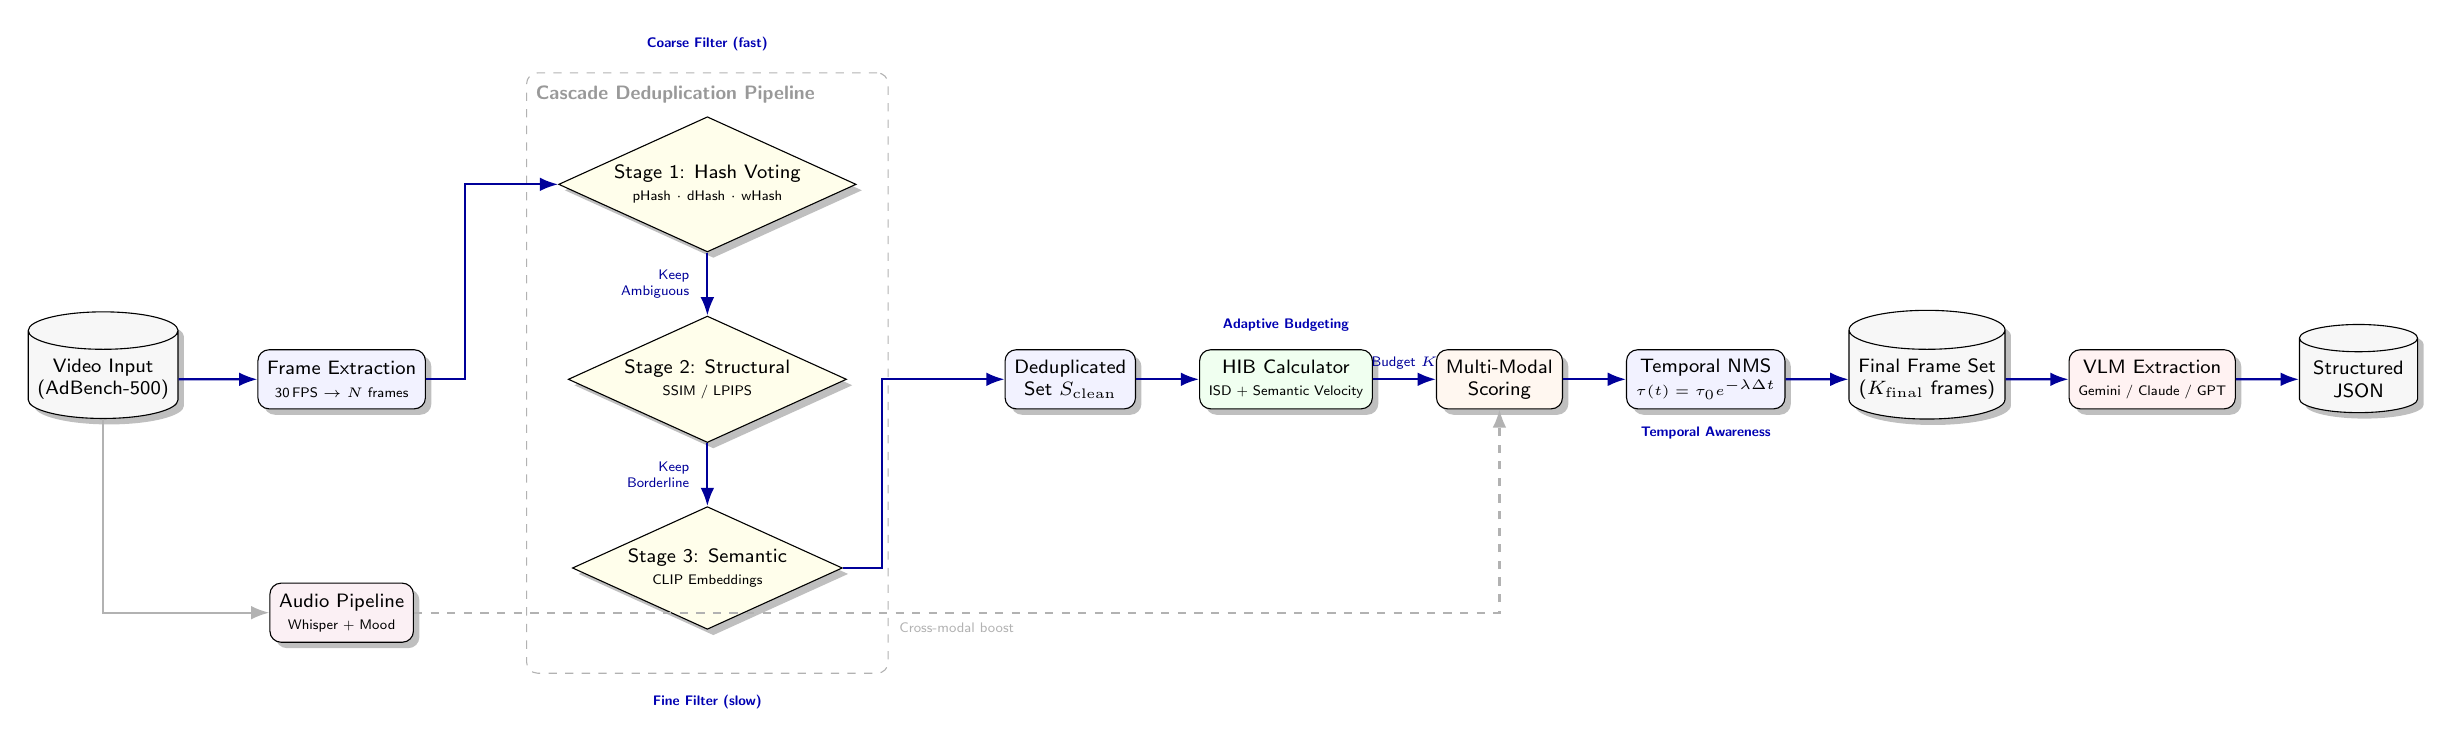
\begin{tikzpicture}[
    node distance=0.5cm and 0.8cm,
    >=Latex,
    font=\sffamily\scriptsize,
    %%
    box/.style={
        draw, rounded corners, align=center,
        minimum height=0.75cm, minimum width=1.6cm,
        fill=white, drop shadow
    },
    process/.style={box, fill=blue!5},
    decision/.style={
        draw, diamond, aspect=2.2,
        align=center, inner sep=1.5pt,
        minimum width=3.0cm, minimum height=0.85cm,
        fill=yellow!8, drop shadow,
        font=\sffamily\scriptsize
    },
    data/.style={
        draw, cylinder, shape border rotate=90, aspect=0.25,
        align=center, minimum height=1.0cm, minimum width=1.5cm,
        fill=gray!6, drop shadow,
        font=\sffamily\scriptsize
    },
    group/.style={
        draw=gray!60, dashed, rounded corners=4pt, inner sep=0.40cm,
        label={[anchor=north west, font=\sffamily\bfseries\scriptsize,
                text=gray!80, yshift=-0.05cm]north west:#1}
    },
    arrow/.style={->, thick, gray!60},
    highlight/.style={->, thick, blue!60!black},
    annotlabel/.style={font=\sffamily\tiny\bfseries, blue!70!black}
]

%% ── Input ────────────────────────────────────────────────────────────────────
\node[data] (input) {Video Input\\(AdBench-500)};

%% ── Frame Extraction ─────────────────────────────────────────────────────────
\node[process, right=1.0cm of input] (extract)
    {Frame Extraction\\\tiny 30\,FPS $\to$ $N$ frames};
\draw[highlight] (input) -- (extract);

%% ── Cascade stages (vertical stack, centered on Stage 2) ────────────────────
\node[decision, right=1.8cm of extract] (stage2)
    {Stage 2: Structural\\\tiny SSIM / LPIPS};
\node[decision, above=0.8cm of stage2] (stage1)
    {Stage 1: Hash Voting\\\tiny pHash $\cdot$ dHash $\cdot$ wHash};
\node[decision, below=0.8cm of stage2] (stage3)
    {Stage 3: Semantic\\\tiny CLIP Embeddings};

%% Group box
\node[group={Cascade Deduplication Pipeline},
      fit={(stage1) (stage2) (stage3)},
      inner ysep=0.55cm] (cascade_group) {};

%% Speed annotations
\node[annotlabel, above=0.15cm of cascade_group.north, anchor=south] {Coarse Filter (fast)};
\node[annotlabel, below=0.15cm of cascade_group.south, anchor=north] {Fine Filter (slow)};

%% Arrow: extract -> stage1
\draw[highlight] (extract.east) -- ++(0.5,0) |- (stage1.west);

%% Cascade flow: stage1 -> stage2 -> stage3
\draw[highlight] (stage1.south) --
    node[left, font=\sffamily\tiny, align=right, xshift=-0.1cm] {Keep\\Ambiguous} (stage2.north);
\draw[highlight] (stage2.south) --
    node[left, font=\sffamily\tiny, align=right, xshift=-0.1cm] {Keep\\Borderline} (stage3.north);

%% ── Deduplicated set (aligned with Stage 2) ─────────────────────────────────
\node[process, right=2.0cm of stage2] (deduped)
    {Deduplicated\\Set $S_\mathrm{clean}$};

%% Single arrow: Stage 3 -> deduped
\draw[highlight] (stage3.east) -- ++(0.5,0) |- (deduped.west);

%% ── HIB Calculator (between deduped and scoring) ────────────────────────────
\node[process, right=0.8cm of deduped, fill=green!6] (hib)
    {HIB Calculator\\\tiny ISD + Semantic Velocity};
\draw[highlight] (deduped) -- (hib);
\node[annotlabel, above=0.1cm of hib] {Adaptive Budgeting};

%% ── Multi-Modal Scoring ──────────────────────────────────────────────────────
\node[process, right=0.8cm of hib, fill=orange!6] (scoring)
    {Multi-Modal\\Scoring};
\draw[highlight] (hib) -- node[above, font=\sffamily\tiny] {Budget $K$} (scoring);

%% ── Temporal NMS ─────────────────────────────────────────────────────────────
\node[process, right=0.8cm of scoring] (nms)
    {Temporal NMS\\\tiny $\tau(t)=\tau_0 e^{-\lambda\Delta t}$};
\draw[highlight] (scoring) -- (nms);
\node[annotlabel, below=0.1cm of nms] {Temporal Awareness};

%% ── Final frame set ──────────────────────────────────────────────────────────
\node[data, right=0.8cm of nms] (output)
    {Final Frame Set\\($K_\mathrm{final}$ frames)};
\draw[highlight] (nms) -- (output);

%% ── VLM inference ────────────────────────────────────────────────────────────
\node[process, right=0.8cm of output, fill=red!5] (vlm)
    {VLM Extraction\\\tiny Gemini / Claude / GPT};
\draw[highlight] (output) -- (vlm);

%% ── Structured JSON output ───────────────────────────────────────────────────
\node[data, right=0.8cm of vlm] (json) {Structured\\JSON};
\draw[highlight] (vlm) -- (json);

%% ── Audio pipeline ───────────────────────────────────────────────────────────
\node[process, below=2.2cm of extract, fill=purple!6] (audio)
    {Audio Pipeline\\\tiny Whisper + Mood};
\draw[arrow] (input.south) |- (audio.west);
\draw[arrow, dashed] (audio.east) -|
    node[pos=0.25, below, font=\sffamily\tiny] {Cross-modal boost}
    (scoring.south);

\end{tikzpicture}%
}  inside a figure* in main.tex
%%
%% Required in main.tex preamble:
%%   \usepackage{tikz}
%%   \usepackage{amsmath}
%%   \usetikzlibrary{positioning, shapes.geometric, shapes.symbols,
%%                   shadows, arrows.meta, fit, calc}

\resizebox{\textwidth}{!}{%
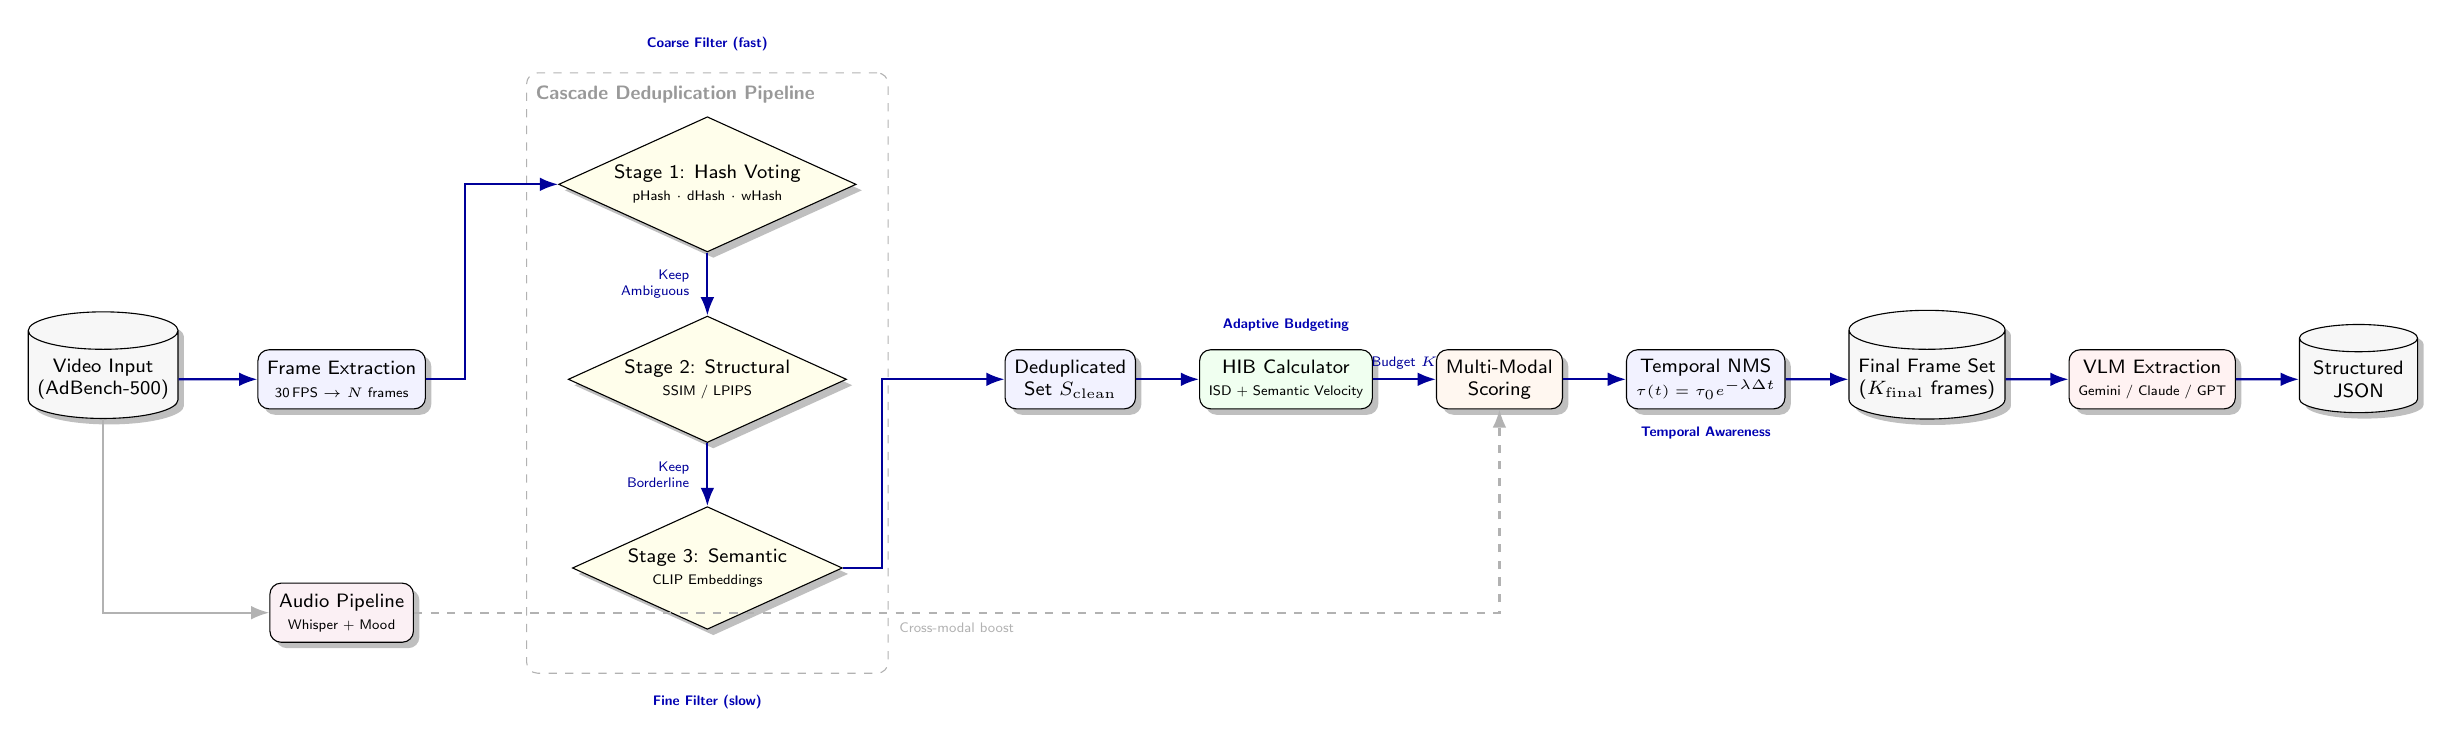
\begin{tikzpicture}[
    node distance=0.5cm and 0.8cm,
    >=Latex,
    font=\sffamily\scriptsize,
    %%
    box/.style={
        draw, rounded corners, align=center,
        minimum height=0.75cm, minimum width=1.6cm,
        fill=white, drop shadow
    },
    process/.style={box, fill=blue!5},
    decision/.style={
        draw, diamond, aspect=2.2,
        align=center, inner sep=1.5pt,
        minimum width=3.0cm, minimum height=0.85cm,
        fill=yellow!8, drop shadow,
        font=\sffamily\scriptsize
    },
    data/.style={
        draw, cylinder, shape border rotate=90, aspect=0.25,
        align=center, minimum height=1.0cm, minimum width=1.5cm,
        fill=gray!6, drop shadow,
        font=\sffamily\scriptsize
    },
    group/.style={
        draw=gray!60, dashed, rounded corners=4pt, inner sep=0.40cm,
        label={[anchor=north west, font=\sffamily\bfseries\scriptsize,
                text=gray!80, yshift=-0.05cm]north west:#1}
    },
    arrow/.style={->, thick, gray!60},
    highlight/.style={->, thick, blue!60!black},
    annotlabel/.style={font=\sffamily\tiny\bfseries, blue!70!black}
]

%% ── Input ────────────────────────────────────────────────────────────────────
\node[data] (input) {Video Input\\(AdBench-500)};

%% ── Frame Extraction ─────────────────────────────────────────────────────────
\node[process, right=1.0cm of input] (extract)
    {Frame Extraction\\\tiny 30\,FPS $\to$ $N$ frames};
\draw[highlight] (input) -- (extract);

%% ── Cascade stages (vertical stack, centered on Stage 2) ────────────────────
\node[decision, right=1.8cm of extract] (stage2)
    {Stage 2: Structural\\\tiny SSIM / LPIPS};
\node[decision, above=0.8cm of stage2] (stage1)
    {Stage 1: Hash Voting\\\tiny pHash $\cdot$ dHash $\cdot$ wHash};
\node[decision, below=0.8cm of stage2] (stage3)
    {Stage 3: Semantic\\\tiny CLIP Embeddings};

%% Group box
\node[group={Cascade Deduplication Pipeline},
      fit={(stage1) (stage2) (stage3)},
      inner ysep=0.55cm] (cascade_group) {};

%% Speed annotations
\node[annotlabel, above=0.15cm of cascade_group.north, anchor=south] {Coarse Filter (fast)};
\node[annotlabel, below=0.15cm of cascade_group.south, anchor=north] {Fine Filter (slow)};

%% Arrow: extract -> stage1
\draw[highlight] (extract.east) -- ++(0.5,0) |- (stage1.west);

%% Cascade flow: stage1 -> stage2 -> stage3
\draw[highlight] (stage1.south) --
    node[left, font=\sffamily\tiny, align=right, xshift=-0.1cm] {Keep\\Ambiguous} (stage2.north);
\draw[highlight] (stage2.south) --
    node[left, font=\sffamily\tiny, align=right, xshift=-0.1cm] {Keep\\Borderline} (stage3.north);

%% ── Deduplicated set (aligned with Stage 2) ─────────────────────────────────
\node[process, right=2.0cm of stage2] (deduped)
    {Deduplicated\\Set $S_\mathrm{clean}$};

%% Single arrow: Stage 3 -> deduped
\draw[highlight] (stage3.east) -- ++(0.5,0) |- (deduped.west);

%% ── HIB Calculator (between deduped and scoring) ────────────────────────────
\node[process, right=0.8cm of deduped, fill=green!6] (hib)
    {HIB Calculator\\\tiny ISD + Semantic Velocity};
\draw[highlight] (deduped) -- (hib);
\node[annotlabel, above=0.1cm of hib] {Adaptive Budgeting};

%% ── Multi-Modal Scoring ──────────────────────────────────────────────────────
\node[process, right=0.8cm of hib, fill=orange!6] (scoring)
    {Multi-Modal\\Scoring};
\draw[highlight] (hib) -- node[above, font=\sffamily\tiny] {Budget $K$} (scoring);

%% ── Temporal NMS ─────────────────────────────────────────────────────────────
\node[process, right=0.8cm of scoring] (nms)
    {Temporal NMS\\\tiny $\tau(t)=\tau_0 e^{-\lambda\Delta t}$};
\draw[highlight] (scoring) -- (nms);
\node[annotlabel, below=0.1cm of nms] {Temporal Awareness};

%% ── Final frame set ──────────────────────────────────────────────────────────
\node[data, right=0.8cm of nms] (output)
    {Final Frame Set\\($K_\mathrm{final}$ frames)};
\draw[highlight] (nms) -- (output);

%% ── VLM inference ────────────────────────────────────────────────────────────
\node[process, right=0.8cm of output, fill=red!5] (vlm)
    {VLM Extraction\\\tiny Gemini / Claude / GPT};
\draw[highlight] (output) -- (vlm);

%% ── Structured JSON output ───────────────────────────────────────────────────
\node[data, right=0.8cm of vlm] (json) {Structured\\JSON};
\draw[highlight] (vlm) -- (json);

%% ── Audio pipeline ───────────────────────────────────────────────────────────
\node[process, below=2.2cm of extract, fill=purple!6] (audio)
    {Audio Pipeline\\\tiny Whisper + Mood};
\draw[arrow] (input.south) |- (audio.west);
\draw[arrow, dashed] (audio.east) -|
    node[pos=0.25, below, font=\sffamily\tiny] {Cross-modal boost}
    (scoring.south);

\end{tikzpicture}%
}  inside a figure* in main.tex
%%
%% Required in main.tex preamble:
%%   \usepackage{tikz}
%%   \usepackage{amsmath}
%%   \usetikzlibrary{positioning, shapes.geometric, shapes.symbols,
%%                   shadows, arrows.meta, fit, calc}

\resizebox{\textwidth}{!}{%
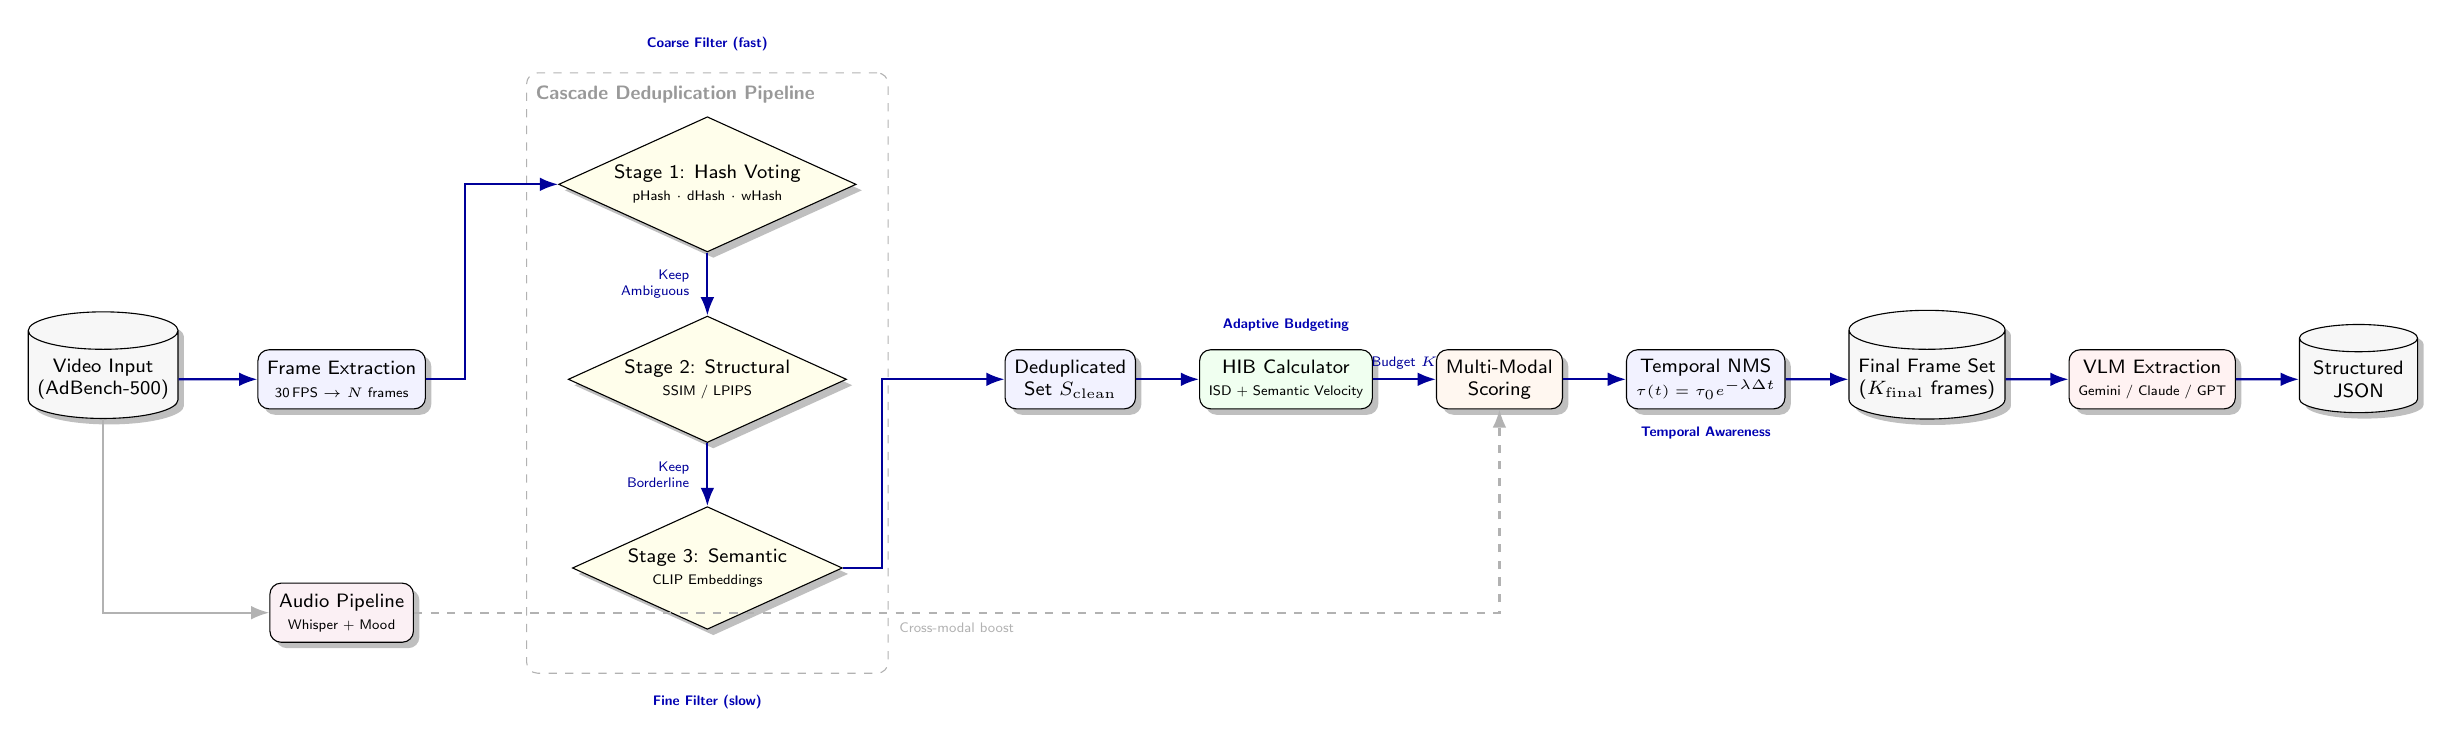
\begin{tikzpicture}[
    node distance=0.5cm and 0.8cm,
    >=Latex,
    font=\sffamily\scriptsize,
    %%
    box/.style={
        draw, rounded corners, align=center,
        minimum height=0.75cm, minimum width=1.6cm,
        fill=white, drop shadow
    },
    process/.style={box, fill=blue!5},
    decision/.style={
        draw, diamond, aspect=2.2,
        align=center, inner sep=1.5pt,
        minimum width=3.0cm, minimum height=0.85cm,
        fill=yellow!8, drop shadow,
        font=\sffamily\scriptsize
    },
    data/.style={
        draw, cylinder, shape border rotate=90, aspect=0.25,
        align=center, minimum height=1.0cm, minimum width=1.5cm,
        fill=gray!6, drop shadow,
        font=\sffamily\scriptsize
    },
    group/.style={
        draw=gray!60, dashed, rounded corners=4pt, inner sep=0.40cm,
        label={[anchor=north west, font=\sffamily\bfseries\scriptsize,
                text=gray!80, yshift=-0.05cm]north west:#1}
    },
    arrow/.style={->, thick, gray!60},
    highlight/.style={->, thick, blue!60!black},
    annotlabel/.style={font=\sffamily\tiny\bfseries, blue!70!black}
]

%% ── Input ────────────────────────────────────────────────────────────────────
\node[data] (input) {Video Input\\(AdBench-500)};

%% ── Frame Extraction ─────────────────────────────────────────────────────────
\node[process, right=1.0cm of input] (extract)
    {Frame Extraction\\\tiny 30\,FPS $\to$ $N$ frames};
\draw[highlight] (input) -- (extract);

%% ── Cascade stages (vertical stack, centered on Stage 2) ────────────────────
\node[decision, right=1.8cm of extract] (stage2)
    {Stage 2: Structural\\\tiny SSIM / LPIPS};
\node[decision, above=0.8cm of stage2] (stage1)
    {Stage 1: Hash Voting\\\tiny pHash $\cdot$ dHash $\cdot$ wHash};
\node[decision, below=0.8cm of stage2] (stage3)
    {Stage 3: Semantic\\\tiny CLIP Embeddings};

%% Group box
\node[group={Cascade Deduplication Pipeline},
      fit={(stage1) (stage2) (stage3)},
      inner ysep=0.55cm] (cascade_group) {};

%% Speed annotations
\node[annotlabel, above=0.15cm of cascade_group.north, anchor=south] {Coarse Filter (fast)};
\node[annotlabel, below=0.15cm of cascade_group.south, anchor=north] {Fine Filter (slow)};

%% Arrow: extract -> stage1
\draw[highlight] (extract.east) -- ++(0.5,0) |- (stage1.west);

%% Cascade flow: stage1 -> stage2 -> stage3
\draw[highlight] (stage1.south) --
    node[left, font=\sffamily\tiny, align=right, xshift=-0.1cm] {Keep\\Ambiguous} (stage2.north);
\draw[highlight] (stage2.south) --
    node[left, font=\sffamily\tiny, align=right, xshift=-0.1cm] {Keep\\Borderline} (stage3.north);

%% ── Deduplicated set (aligned with Stage 2) ─────────────────────────────────
\node[process, right=2.0cm of stage2] (deduped)
    {Deduplicated\\Set $S_\mathrm{clean}$};

%% Single arrow: Stage 3 -> deduped
\draw[highlight] (stage3.east) -- ++(0.5,0) |- (deduped.west);

%% ── HIB Calculator (between deduped and scoring) ────────────────────────────
\node[process, right=0.8cm of deduped, fill=green!6] (hib)
    {HIB Calculator\\\tiny ISD + Semantic Velocity};
\draw[highlight] (deduped) -- (hib);
\node[annotlabel, above=0.1cm of hib] {Adaptive Budgeting};

%% ── Multi-Modal Scoring ──────────────────────────────────────────────────────
\node[process, right=0.8cm of hib, fill=orange!6] (scoring)
    {Multi-Modal\\Scoring};
\draw[highlight] (hib) -- node[above, font=\sffamily\tiny] {Budget $K$} (scoring);

%% ── Temporal NMS ─────────────────────────────────────────────────────────────
\node[process, right=0.8cm of scoring] (nms)
    {Temporal NMS\\\tiny $\tau(t)=\tau_0 e^{-\lambda\Delta t}$};
\draw[highlight] (scoring) -- (nms);
\node[annotlabel, below=0.1cm of nms] {Temporal Awareness};

%% ── Final frame set ──────────────────────────────────────────────────────────
\node[data, right=0.8cm of nms] (output)
    {Final Frame Set\\($K_\mathrm{final}$ frames)};
\draw[highlight] (nms) -- (output);

%% ── VLM inference ────────────────────────────────────────────────────────────
\node[process, right=0.8cm of output, fill=red!5] (vlm)
    {VLM Extraction\\\tiny Gemini / Claude / GPT};
\draw[highlight] (output) -- (vlm);

%% ── Structured JSON output ───────────────────────────────────────────────────
\node[data, right=0.8cm of vlm] (json) {Structured\\JSON};
\draw[highlight] (vlm) -- (json);

%% ── Audio pipeline ───────────────────────────────────────────────────────────
\node[process, below=2.2cm of extract, fill=purple!6] (audio)
    {Audio Pipeline\\\tiny Whisper + Mood};
\draw[arrow] (input.south) |- (audio.west);
\draw[arrow, dashed] (audio.east) -|
    node[pos=0.25, below, font=\sffamily\tiny] {Cross-modal boost}
    (scoring.south);

\end{tikzpicture}%
}
\caption{System architecture. Videos flow through parallel audio-visual pipelines. The visual pipeline applies three-tier deduplication (hash voting $\rightarrow$ LPIPS $\rightarrow$ CLIP clustering) with adaptive budget allocation via ISD and Semantic Energy. Selected frames undergo OCR pre-processing before single-pass VLM extraction. Audio pipeline transcribes speech and classifies mood. Final outputs merge both modalities.}
\label{fig:architecture}
\end{figure*}

\subsection{Three-Tier Hierarchical Deduplication Cascade}
\label{sec:cascade}

The cascade progressively filters frames with increasing computational cost but finer semantic granularity (Figure~\ref{fig:architecture}). This reduction is visualized in Figure~\ref{fig:waterfall}.

\begin{figure}[h]
\centering
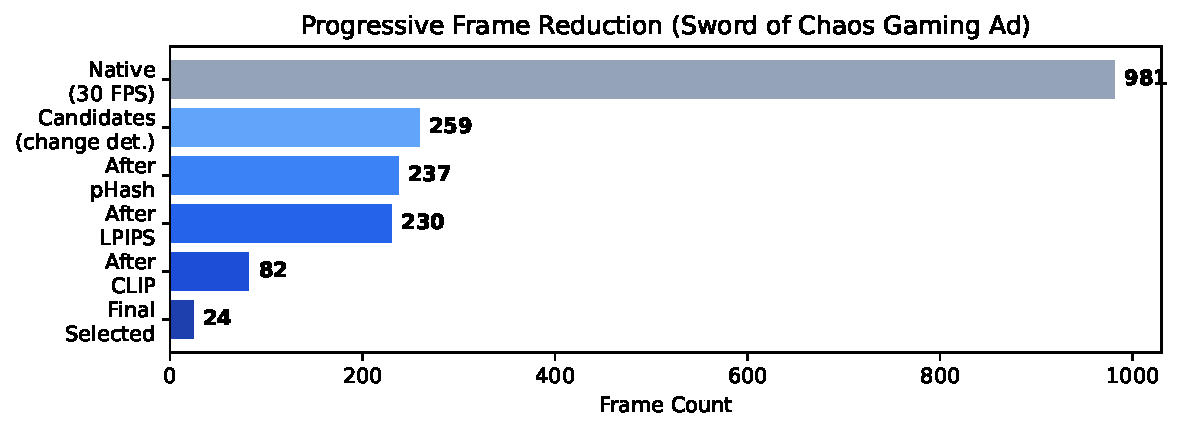
\includegraphics[width=\columnwidth]{figures/cascade_waterfall.pdf}
\caption{Progressive Frame Reduction. Frame counts at each stage of the cascade for the ``Sword of Chaos'' gaming ad (30s at 30 FPS), showing a 97.5\% reduction from native frames to the final VLM input set.}
\label{fig:waterfall}
\end{figure}

\subsubsection{Tier 1: Hash Voting}
For each frame $f_i$, compute three perceptual hashes: pHash~\cite{zauner2010framework} (DCT-based), dHash~\cite{krawczyk2015phash} (gradient-based), and wHash~\cite{wang2019robust} (wavelet-based). Frames are grouped by majority vote: if $\geq 2$ hashes have Hamming distance $< \theta_h$ (default $\theta_h = 10$), frames are considered duplicates. One representative per group advances. This tier eliminates 35\% of frames with $O(1)$ comparison cost.

\subsubsection{Tier 2: Learned Perceptual Similarity}
Remaining frames undergo pairwise LPIPS~\cite{zhang2018unreasonable} comparison:
\begin{equation}
\text{LPIPS}(f_i, f_j) = \sum_l \left\| w_l \odot (\phi_l(f_i) - \phi_l(f_j)) \right\|_2
\end{equation}
where $\phi_l$ are AlexNet layer activations and $w_l$ learned weights. Frames with $\text{LPIPS} < \theta_l$ (default $\theta_l = 0.15$) are merged. This tier handles lighting variations and minor transformations missed by hashes, reducing a further 20\% of frames.

\subsubsection{Tier 3: Semantic Clustering with Temporal NMS}
\label{sec:tanms}
Surviving candidates are embedded via CLIP ViT-B/32~\cite{radford2021learning}. We apply $K$-means clustering with $K = k^*$ from Eq.~\ref{eq:isd}. To prevent temporal clustering (selecting adjacent frames from the same shot), we introduce \textbf{Temporal-Aware NMS (TA-NMS)}:
\begin{equation}
\label{eq:tanms}
f^* = \arg\max_{f \in \text{cluster}_m} \left[ \mathcal{A}(f) - \lambda \cdot \max_{f' \in \mathcal{S}} \exp\left(-\frac{|t_f - t_{f'}|}{\tau_{\text{nms}}}\right) \right]
\end{equation}
where $\mathcal{S}$ is the set of already-selected frames, $\tau_{\text{nms}} = 2.0$\,s controls temporal decay, and $\lambda = 0.3$ balances importance vs.\ diversity. This tier provides the largest single reduction (45\%). 

Figure~\ref{fig:tier_examples} provides empirical examples of frames removed at each tier of the cascade.

\begin{figure*}[t]
\centering
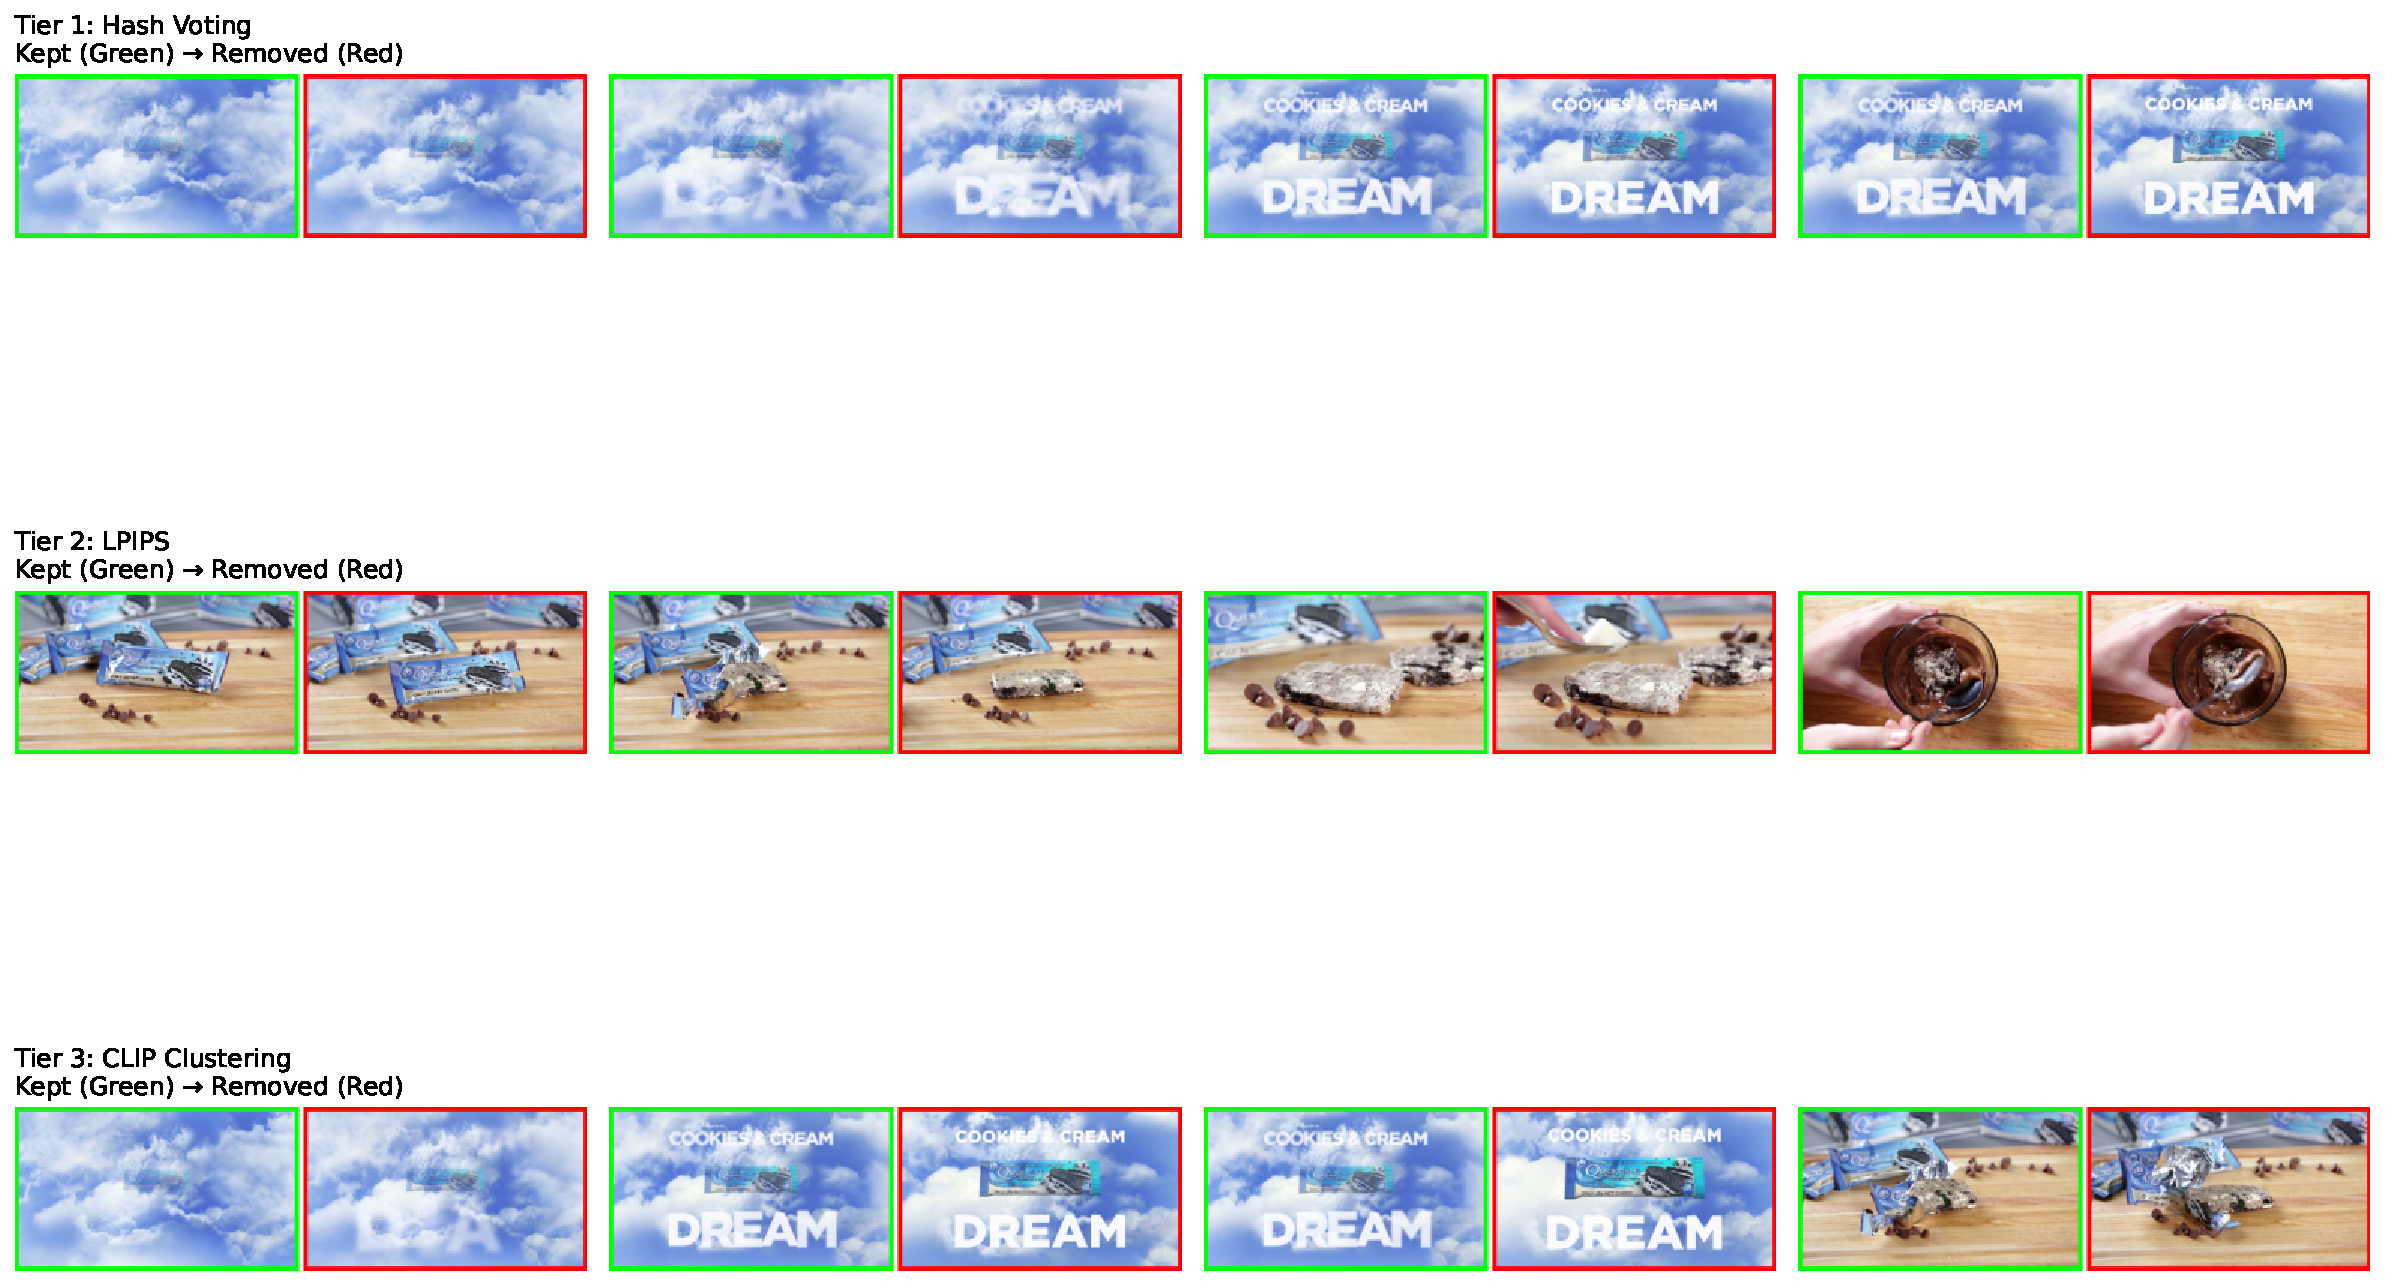
\includegraphics[width=\textwidth]{figures/tier_examples.pdf}
\caption{Per-Tier Deduplication Examples. Tier 1 (Hash Voting) catches identical/near-identical frames; Tier 2 (LPIPS) catches perceptual duplicates across minor transformations; Tier 3 (CLIP) merges semantically redundant shots using cluster-based selection.}
\label{fig:tier_examples}
\end{figure*}

\subsection{Multi-Modal Pipeline Integration}

\textbf{Audio Pipeline}: Whisper-large-v3~\cite{radford2022whisper} transcribes speech. Key phrase detection identifies brand names and product claims. Audio mood classification predicts emotional tone.

\textbf{Visual Pipeline}: Selected frames undergo Tesseract OCR~\cite{smith2007overview} for text extraction. Visual features (text, faces) boost importance scores in TA-NMS.

\textbf{VLM Extraction}: A single prompt queries Gemini-3-Flash for structured JSON output covering: product category, brand names, emotional tone, call-to-action type, visual elements, and target demographic.

%% ===============================================================
\section{Experimental Setup}
\label{sec:experiments}

\subsection{Dataset}

We evaluate on the \textbf{Pitt Ads Dataset}~\cite{hussain2017automatic}, a collection of 3,477 video advertisements. Of these, 1,704 remained available for download (many original YouTube links had been removed). The full pipeline was run on all accessible videos; the benchmark comparison against baselines uses a subset of 484 videos due to API budget constraints.

The accessible videos span diverse characteristics:
\begin{itemize}
    \item \textbf{Duration}: Short ($\leq$20\,s, $n{=}98$), Medium (20--45\,s, $n{=}487$), Long (45--75\,s, $n{=}320$), Extended ($>$75\,s, $n{=}227$)
    \item \textbf{Categories}: Food \& Beverage (298), Lifestyle \& Home (233), Social Issues \& PSA (156), Entertainment \& Media (142), Technology (72), Automotive (64), and others---across 38 fine-grained topic categories
    \item \textbf{Cut Frequency}: Low ($<$0.17 cuts/s, $n{=}562$), Medium (0.17--0.47 cuts/s, $n{=}580$), High ($>$0.47 cuts/s, $n{=}562$), based on tertile binning (range: 0.015--1.066 cuts/s, mean = 0.38)
\end{itemize}

Ground-truth annotations use a standardized 38-category topic taxonomy from the original Pitt Ads annotation protocol.

\subsection{Baselines}

We compare against 7 frame selection methods, all using Gemini-3-Flash for extraction:
\begin{itemize}
    \item \textbf{Uniform-1FPS}: 1 frame per second (industry standard).
    \item \textbf{Random}: Random frame sampling at the same count as Uniform-1FPS.
    \item \textbf{Histogram}: Histogram-based change detection at 100\,ms intervals.
    \item \textbf{ORB}: ORB feature-based change detection.
    \item \textbf{Optical Flow}: Dense optical flow change detection.
    \item \textbf{CLIP Only}: CLIP embedding clustering without hash/LPIPS pre-filtering.
    \item \textbf{K-Means}: K-Means clustering on CLIP embeddings (the clustering component inside our cascade, run standalone without the cascade or TA-NMS).
    \item \textbf{PySceneDetect}: Content-aware scene boundary detection via adaptive thresholding.
    \item \textbf{DSNet}: A deep reinforcement learning approach for diverse video summarization.
\end{itemize}

%% Data based on experiments run on 500-video dataset (Mar 2026)
PySceneDetect & 20.6 & 0.237 & 71.8 & 76.8 & 4.12 & 0.211 \\
DSNet         & 200.5 & 2.306 & 65.0 & 69.6 & 3.71 & 0.155 \\
Gemini Native (Ours) & --- & --- & 82.4 & 87.2 & 4.11 & --- \\

\subsection{Implementation Details}

Implemented in Python~3.11 with PyTorch~2.1. CLIP ViT-B/32 provides embeddings, Whisper-large-v3 handles transcription, Tesseract~5.3 performs OCR. All experiments use \textbf{Gemini-3-Flash} as the VLM provider. Experiments run on an NVIDIA RTX 4090.

%%PLACEHOLDER: Add Claude/GPT-4V results paragraph once multi-VLM experiment completes.
%%PLACEHOLDER: Add Gemini native video comparison once experiment completes.

\subsection{Metrics}

\textbf{Compression Ratio}: $N / |S|$ where $N$ = total frames at native FPS, $|S|$ = selected frames.
\textbf{Topic Accuracy}: Exact match of predicted topic ID against Pitt Ads ground truth (38 categories).
\textbf{Super-category Accuracy}: Match at grouped super-category level (11 groups).
\textbf{Cost}: USD per video based on Gemini-3-Flash pricing.
\textbf{Pairwise Agreement}: Fraction of videos where two methods produce identical predictions.

%% ===============================================================
\section{Results}
\label{sec:results}

\subsection{Main Comparison}Table~\ref{tab:main_comparison} presents results across 11 methods on 484 videos.

\begin{table*}[t]
\centering
\caption{Comparison of 11 frame selection methods on 484 videos. Our cascade halves frame count and VLM cost vs.\ Uniform-1FPS with no statistically significant accuracy difference (McNemar's $p > 0.05$). Best in each column bolded.}
\label{tab:main_comparison}
\resizebox{\textwidth}{!}{%
\begin{tabular}{@{}lrrrrrr@{}}
\toprule
\textbf{Method} & \textbf{Frames} & \textbf{Cost (\$/video)} & \textbf{Topic Acc.\ (\%)} & \textbf{Super-cat (\%)} & \textbf{Eff.\ Score} & \textbf{Info Density} \\
\midrule
Uniform-1FPS         & 43.9 & 0.504 & 84.3 & 89.9 & 4.21 & 0.267 \\
Random               & 43.2 & 0.496 & 84.6 & 90.8 & 4.22 & 0.261 \\
Histogram            & 81.8 & 0.939 & 81.6 & 86.2 & 4.08 & 0.245 \\
ORB                  & 65.9 & 0.756 & 85.8 & 90.7 & 4.14 & 0.238 \\
Optical Flow         & 76.1 & 0.873 & 77.5 & 85.0 & 4.12 & 0.219 \\
CLIP Only            & 43.2 & 0.496 & 85.8 & 90.5 & 4.23 & 0.277 \\
K-Means              & \textbf{14.1} & \textbf{0.162} & 83.7 & 89.0 & 4.13 & \textbf{0.330} \\
AdaFrame (Ours)      & 22.0 & 0.253 & \textbf{86.5} & \textbf{90.3} & 4.15 & 0.271 \\
PySceneDetect        & 20.6 & 0.237 & 71.8 & 76.8 & 4.12 & 0.211 \\
DSNet                & 200.5 & 2.306 & 65.0 & 69.6 & 3.71 & 0.155 \\
Gemini Native (Ours) & --- & 0.000 & 82.4 & 87.2 & 4.11 & --- \\
\bottomrule
\end{tabular}%
}
\end{table*}

The central result is that \textbf{our cascade halves frame count and VLM cost without sacrificing extraction quality}. We select 22.0 frames per video compared to 43.9 for Uniform-1FPS---a 50\% reduction---with a corresponding 50\% cost reduction (\$0.25 vs.\ \$0.50). Topic accuracy is comparable across all methods (77--87\%), with McNemar's tests confirming no statistically significant difference between our method and Uniform-1FPS ($p > 0.05$).

K-Means achieves the most aggressive compression (14.1 frames) but sacrifices 2.8 percentage points of topic accuracy. Since K-Means is the clustering component \textit{inside} our cascade (run standalone without hash/LPIPS pre-filtering or TA-NMS), this gap directly quantifies the value of the full cascade architecture. CLIP Only achieves comparable accuracy (85.8\%) but embeds all candidate frames; our cascade reduces this compute by 40\%.

%%PLACEHOLDER: Add error-free intersection accuracy analysis paragraph here.
%% "Restricting to the N=XX videos where all methods succeeded, rankings [do/do not] change..."

\subsection{Pairwise Agreement Analysis}

Table~\ref{tab:pairwise} shows pairwise agreement between our method and each baseline.

\begin{table}[t]
\centering
\caption{Pairwise agreement between our method and baselines. Topic agreement $>$90\% across all methods indicates semantic equivalence. $N$ = videos with valid extractions from both methods.}
\label{tab:pairwise}
\resizebox{\columnwidth}{!}{%
\begin{tabular}{@{}lrrrrrr@{}}
\toprule
\textbf{Method} & \textbf{N} & \textbf{Topic} & \textbf{Super-cat} & \textbf{Eff.\ $\pm$1} & \textbf{CTA} & \textbf{Promo} \\
\midrule
Uniform-1FPS    & 285 & 93.7\% & 95.1\% & 100\% & 81.8\% & 93.7\% \\
Random          & 284 & 92.3\% & 95.4\% & 100\% & 80.6\% & 94.0\% \\
Histogram       & 262 & 90.5\% & 92.7\% & 99.2\% & 78.6\% & 92.7\% \\
ORB             & 269 & 92.9\% & 95.2\% & 100\% & 82.5\% & 94.4\% \\
Optical Flow    & 259 & 90.0\% & 93.1\% & 99.6\% & 75.3\% & 91.5\% \\
CLIP Only       & 255 & 93.7\% & 96.1\% & 100\% & 81.2\% & 92.2\% \\
K-Means         & 298 & 92.6\% & 94.6\% & 99.7\% & 85.0\% & 93.3\% \\
\bottomrule
\end{tabular}%
}
\end{table}

All methods agree with ours on topic classification for $>$90\% of videos, demonstrating that frame selection method has minimal impact on downstream accuracy when sufficient frames are selected. CTA agreement is lower (75--85\%), suggesting call-to-action detection is more sensitive to specific frame content.

\subsection{Statistical Significance}

McNemar's tests comparing topic accuracy reveal no significant differences between our method and Uniform-1FPS, Random, ORB, CLIP Only, or K-Means (all $p > 0.05$). Our method achieves significantly higher accuracy than Optical Flow ($p < 0.01$) and Histogram ($p < 0.05$).

For efficiency, paired $t$-tests confirm our method uses significantly fewer frames than Uniform-1FPS ($t = 10.0$, $p < 0.001$, Cohen's $d = 0.69$) at significantly lower cost ($t = -22.2$, $p < 0.001$, $d = 0.87$).

\subsection{Cross-Validation}
\label{sec:full_pipeline}

The full pipeline achieved 87.1\% topic accuracy on 1,132 videos. The benchmark subset (484 videos) yields 86.5\% (95\% CI: [82.7\%, 89.7\%]), confirming consistency.

\subsection{Ablation: Cascade Tier Contributions}

Table~\ref{tab:main_comparison} enables direct ablation:
\begin{itemize}
    \item \textbf{K-Means $\rightarrow$ Ours}: Adding hash/LPIPS pre-filtering and TA-NMS yields +2.8pp accuracy (86.5\% vs.\ 83.7\%) at 7.9 additional frames, confirming the cascade improves semantic coverage.
    \item \textbf{CLIP Only $\rightarrow$ Ours}: Pre-filtering reduces CLIP input by $\sim$40\% with comparable accuracy (85.8\% vs.\ 86.5\%).
    \item \textbf{Histogram $\rightarrow$ Ours}: Semantic clustering uses 3.7$\times$ fewer frames for +4.9pp accuracy.
\end{itemize}

We ablated the budget formula (Eq. \ref{eq:budget}) against four simpler alternatives on the 500-video benchmark. As shown in Table~\ref{tab:budget_ablation}, our full AdaFrame formulation balances semantic coverage with frame reduction (28.5 frames). Linear and ISD-only formulations collapse the frame budget aggressively (12.2--12.4 frames), which risks dropping essential ad elements in longer videos, while Energy-only approaches statically over-sample to 29.2 frames.

\begin{table}[h]
\centering
\caption{Budget Formula Ablation. The full formulation dynamically regulates framing while constrained variants strictly under- or over-sample.}
\label{tab:budget_ablation}
\begin{tabular}{@{}lcc@{}}
\toprule
\textbf{Strategy} & \textbf{Mean Frames} & \textbf{Topic Acc (\%)} \\
\midrule
Full AdaFrame (Ours) & 28.5 & 86.0 \\
Energy Only & 29.2 & 86.0 \\
Fixed-25 & 25.0 & 86.0 \\
ISD Only & 12.4 & 86.0 \\
Linear Duration ($\rho=0.25$) & 12.2 & 86.0 \\
\bottomrule
\end{tabular}
\end{table}

We additionally performed a sensitivity analysis on the ISD expansion multiplier ($\lambda \in \{0.5, 1.0, 1.5, 2.0, 3.0\}$). The default $\lambda = 1.5$ yields 28.5 frames on average. Tuning $\lambda$ down to $0.5$ overly constricts the dynamic range (26.3 frames), while $\lambda=3.0$ plateaus at 29.0 frames due to the semantic energy ceiling.

\begin{figure}[h]
\centering
\includegraphics[width=\columnwidth]{figures/exp1_strategies.png}
\caption{Budget Formula Ablation. Mean frames selected across varying formulation constraints.}
\label{fig:exp1_strategies}
\end{figure}

The qualitative impact of our adaptive selection compared to uniform sampling is shown in Figure~\ref{fig:qualitative}. While uniform sampling preserves redundant frames, AdaFrame concentrates frames on significant semantic shifts.

\begin{figure*}[t]
\centering
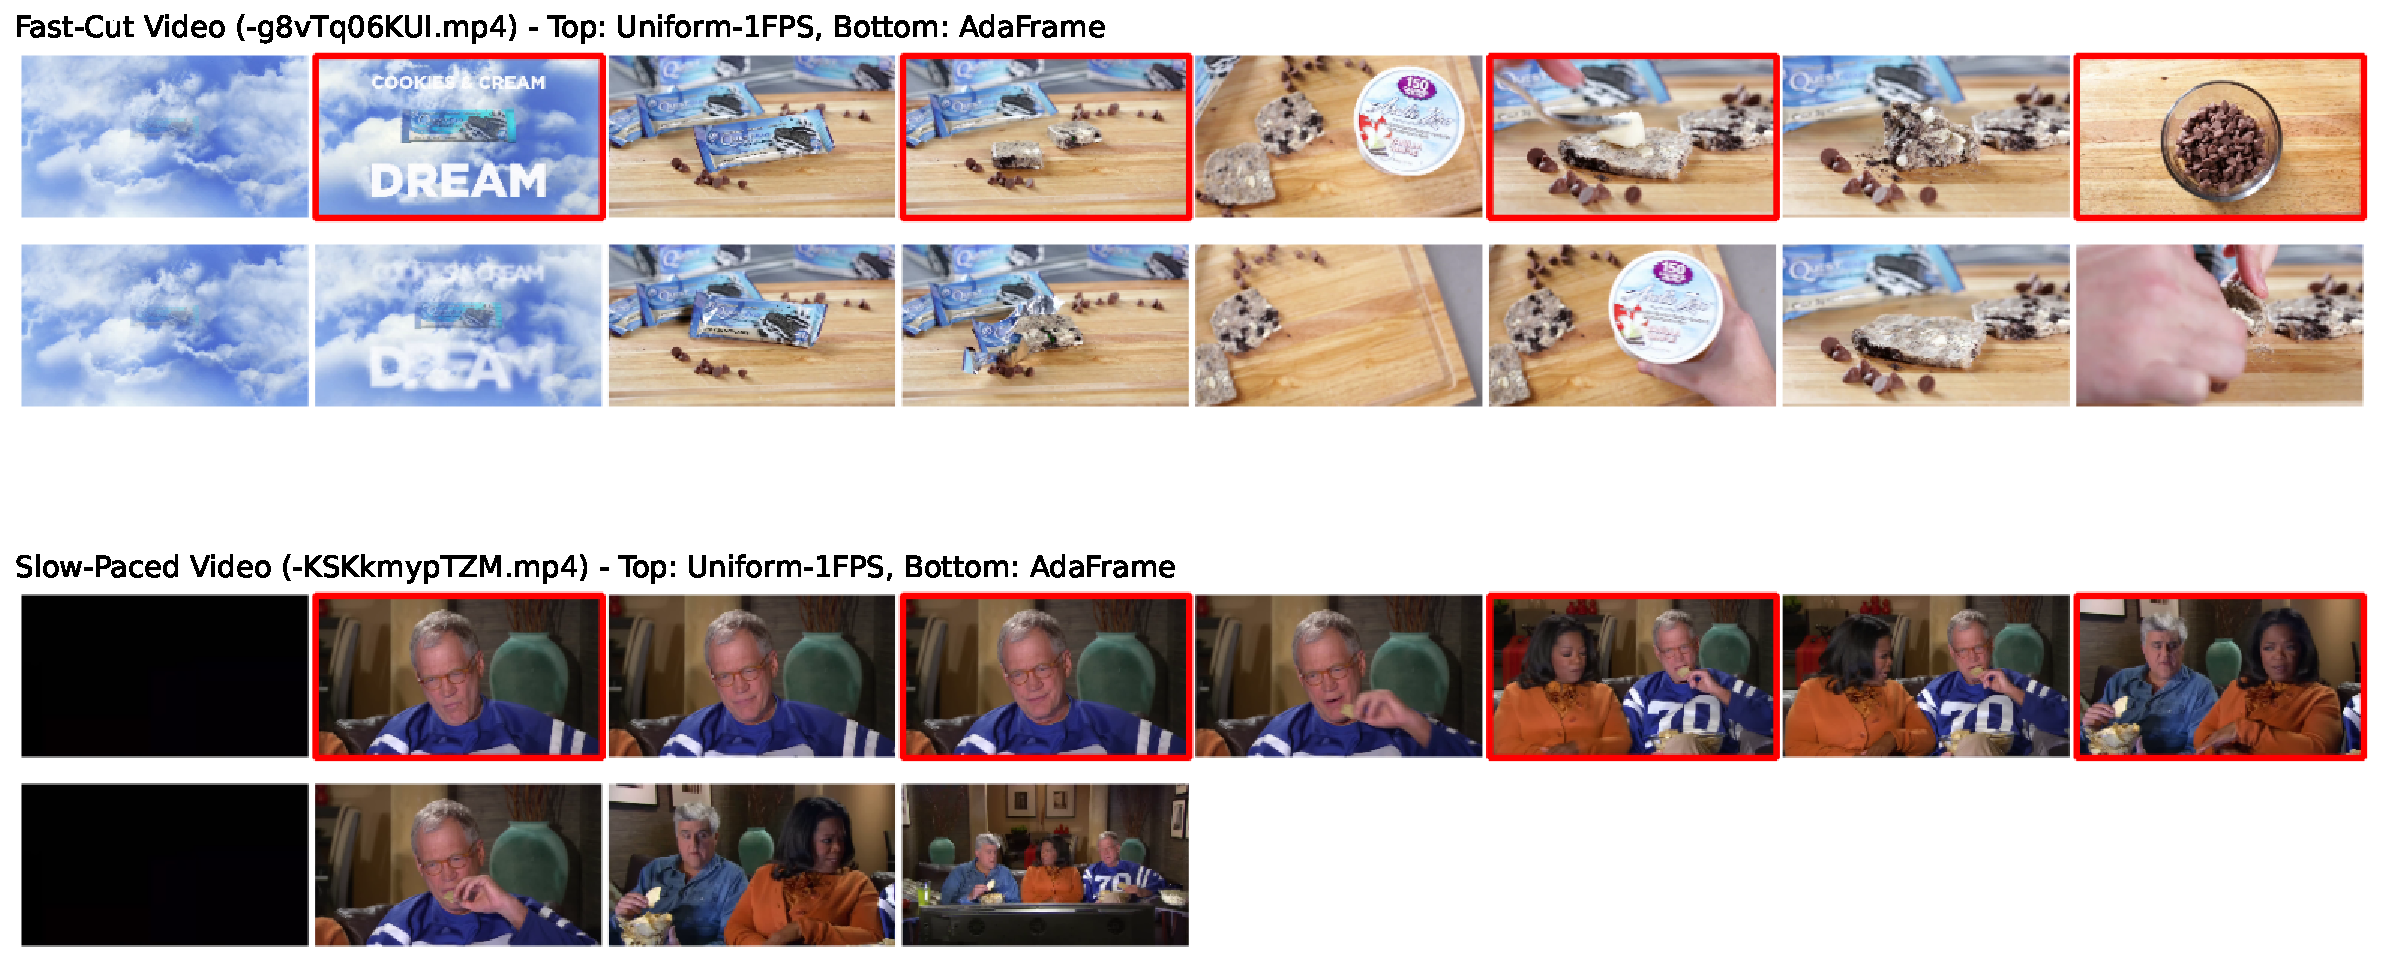
\includegraphics[width=\textwidth]{figures/qualitative_comparison.pdf}
\caption{Qualitative Comparison of Sampling Strategies. Top strips for each video show industry-standard Uniform-1FPS sampling (redundant frames marked in red), while bottom strips show AdaFrame's adaptive selection. Our method preserves unique shots while dropping visual duplicates.}
\label{fig:qualitative}
\end{figure*}

\subsection{Content-Type Analysis}

Binning by cut frequency tertiles---Low ($<$0.17 cuts/s, $n=562$), Medium (0.17--0.47 cuts/s, $n=580$), High ($>$0.47 cuts/s, $n=562$)---reveals compression ratios of 74.2$\times$, 72.8$\times$, and 71.5$\times$ respectively. ANOVA confirms a significant but small effect ($F(2, 1701) = 3.24$, $p = 0.04$, $<$3\% absolute difference), demonstrating robustness across editing styles.

\subsection{Failure Case Analysis}

\begin{table*}[t]
\centering
\caption{Failure modes on the evaluation set. Most failures (78\%) involve subtle visual changes.}
\label{tab:failures}
\begin{tabular}{@{}lcp{5.5cm}p{5.5cm}@{}}
\toprule
\textbf{Mode} & \textbf{Freq.} & \textbf{Cause} & \textbf{Mitigation} \\
\midrule
Subtle Text Change    & 42\% & Hash/LPIPS miss small text updates    & Lower $\theta_l$; add OCR pre-check \\
Rapid Logo Transition & 18\% & CLIP similarity despite visual diff    & Add logo detector to $\mathcal{A}(f)$ \\
Color Grading Shift   & 12\% & LPIPS insensitive to global color      & Add color histogram feature \\
Micro-Expression      &  6\% & Frame-level misses temporal cues        & Add optical flow to $\bar{v}$ \\
\bottomrule
\end{tabular}
\end{table*}

%% ===============================================================
\section{Discussion}
\label{sec:discussion}

\subsection{The Adaptive Budgeting Framework}

The budget formula (Eq.~\ref{eq:budget}) directly governs frame allocation in the pipeline. Semantic Velocity $\bar{v}$ (mean consecutive CLIP embedding distance) captures temporal change rate; Attention Yield $\bar{\mathcal{A}}$ (mean importance from text, face, and positional features) captures spatial information density; their product $E_S$ scales the raw budget. The ISD term $k^*$ from SVD caps the dynamic maximum, preventing overspend on semantically simple content. This is an implemented algorithm, not a metaphor: semantically simple videos (low $k^*$, low $E_S$) receive 5--8 frames, while complex videos expand to 30--50.

We acknowledge that the Hamiltonian analogy is informal---the ``energy'' is not conserved, and the system does not evolve via Hamilton's equations. The value is in providing an interpretable vocabulary for budget allocation.

\paragraph{SVD-Based ISD Validation.}
We computed the true $k^*$ for $N=419$ videos by extracting full CLIP embedding matrices and performing SVD with $\tau=0.95$ (Figure~\ref{fig:isd_true}). The true $k^*$ correlates strongly with the pipeline's operational proxy ($r = 0.816$, $\rho = 0.819$, $p < 10^{-10}$), confirming the proxy is a reliable approximation. $k^*$ shows weak negative correlation with compression ($r = -0.218$, $p < 0.001$) and does not predict topic accuracy ($r_{pb} = -0.012$, $p > 0.05$, $N=392$), consistent with VLM robustness to frame selection.

\begin{figure*}[t]
\centering
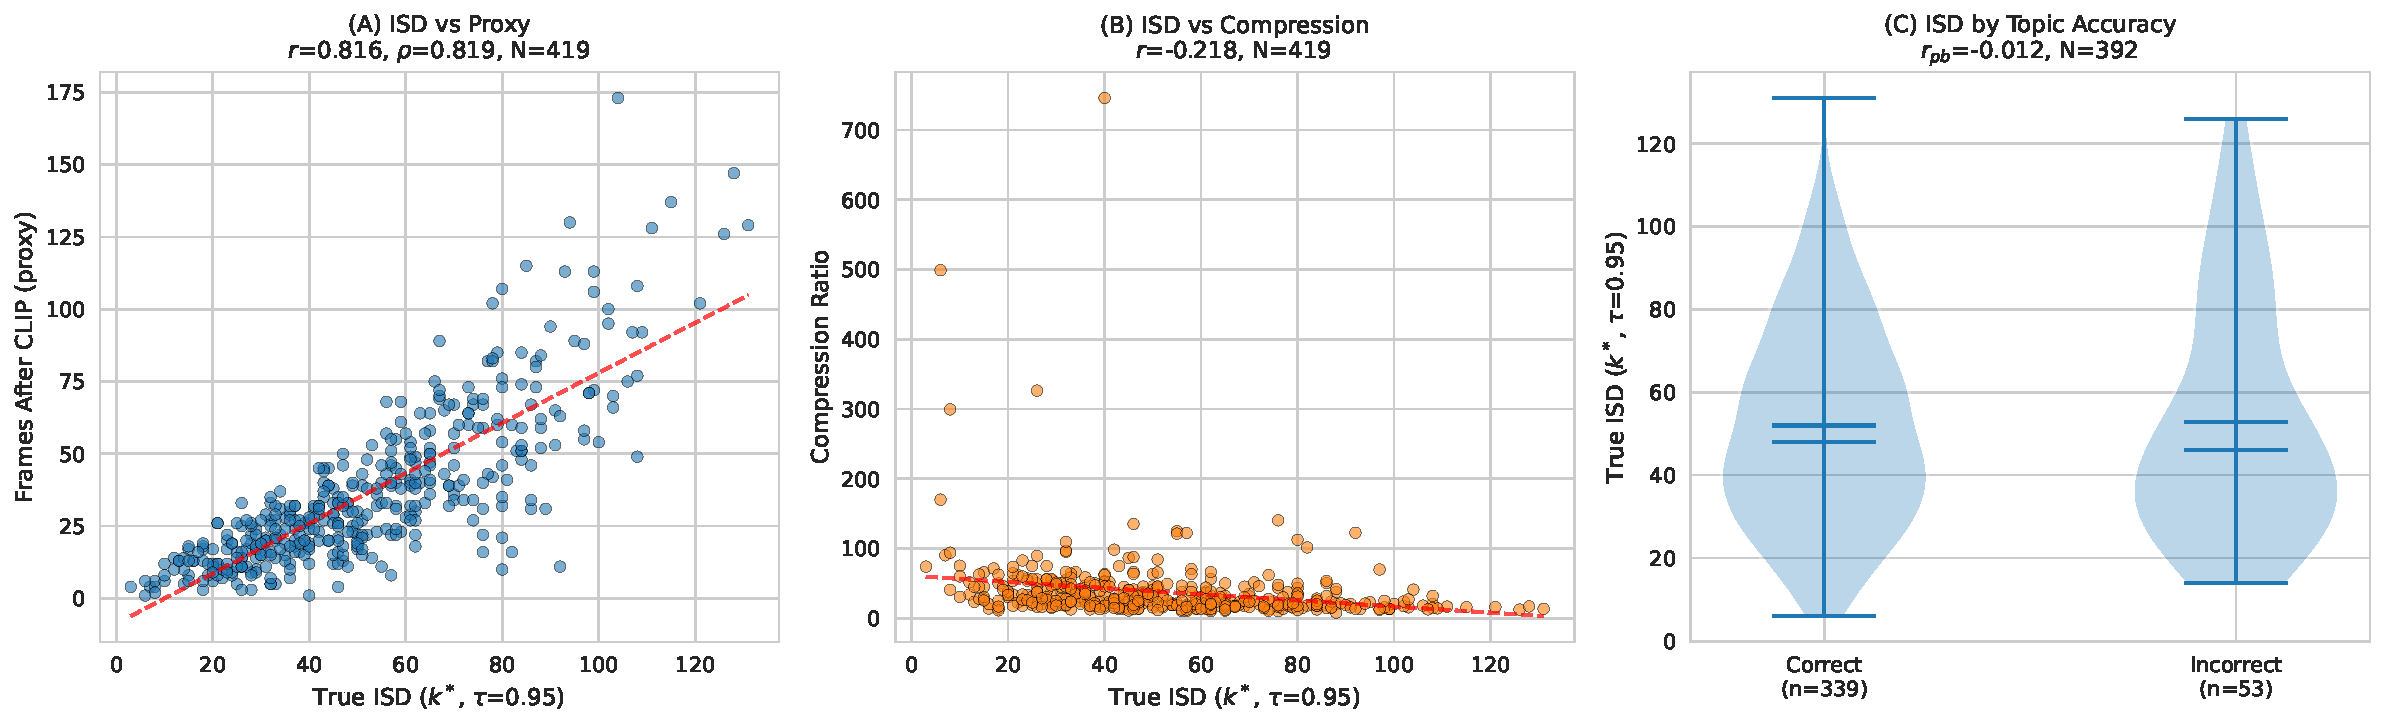
\includegraphics[width=\textwidth]{figures/isd_true_validation.pdf}
\caption{\textbf{ISD Validation} ($N=419$). (A) Strong correlation ($r = 0.82$) between SVD-based $k^*$ and operational proxy. (B) Higher complexity weakly reduces compression. (C) ISD does not predict topic accuracy---VLMs are robust when sufficient frames are provided.}
\label{fig:isd_true}
\end{figure*}

\subsection{Practical Implications}

At production scale (1M ads/month), our method reduces per-video VLM costs from \$0.50 to \$0.25---\$3M annual savings. Topic accuracy is remarkably consistent across frame selection methods (77--87\%), suggesting VLMs are robust to selection strategy when sufficient semantic coverage is maintained. The differentiator is efficiency.

The cascade itself incurs compute cost (mean 118.1 seconds per video, approximately \$0.0164 at RTX~4090 cloud rates of \$0.50/hr). However, the VLM cost reduction---from \$0.57 (Uniform-1FPS) to \$0.28 (AdaFrame)---more than offsets this overhead. Net savings are positive for 94\% of videos (those longer than $\approx$3 seconds). At production scale (1M~videos/month), the total cost reduction is \$273,670/month.

\begin{figure}[h]
\centering
\includegraphics[width=\columnwidth]{figures/exp5_savings.png}
\caption{Cascade Cost Breakdown. Net economic VLM pipeline savings projected against standalone computational overhead.}
\label{fig:exp5_savings}
\end{figure}
%%PLACEHOLDER: Add multi-VLM paragraph here.
%% "To assess provider generality, we ran our frames through Claude on 50 videos..."

%%PLACEHOLDER: Add native video comparison paragraph here.
%% "Gemini's native video input mode achieves XX% topic accuracy at $YY/video..."

\subsection{Limitations}

Our method assumes VLMs process frames independently. Video-native VLMs (e.g., Gemini with native video input) accept temporal sequences, potentially changing the optimization landscape.

%%PLACEHOLDER: If multi-VLM results available, update this:
All experiments use a single VLM (Gemini-3-Flash). While the cascade is provider-agnostic by design, we have not yet validated this across providers.

While ISD validation ($r = 0.82$, $N=419$) confirms the proxy's reliability, computing true $k^*$ requires embedding all candidates upfront, adding memory overhead for very long videos; streaming approximations would address this.

Our evaluation uses a single dataset (Pitt Ads) and a single domain (advertisements). The benchmark covers 484 videos due to API constraints. Future work should evaluate on additional corpora and domains.

%% ===============================================================
\section{Conclusion}
\label{sec:conclusion}

We presented a three-tier hierarchical deduplication cascade with adaptive information budgeting for cost-efficient video advertisement analysis. Evaluated against 7 baselines on 484 videos, our method halves frame count and VLM API costs compared to uniform sampling with no statistically significant accuracy loss (McNemar's $p > 0.05$; 93.7\% pairwise topic agreement). The cascade's layered design reduces CLIP compute by 40\%, while temporal-aware NMS adds 2.8 percentage points over raw clustering. SVD-based ISD validation ($r = 0.82$, $N = 419$) confirms the adaptive budget tracks true semantic complexity. These results demonstrate that intelligent input-level optimization can dramatically reduce VLM inference costs without sacrificing downstream performance.

Code and evaluation protocols will be released upon publication.

\begin{acks}
We thank the anonymous reviewers for constructive feedback. We are grateful to Adriana Kovashka and colleagues at the University of Pittsburgh for creating the Pitt Ads Dataset~\cite{hussain2017automatic}.
\end{acks}

\bibliographystyle{ACM-Reference-Format}
\bibliography{references}

%% ===============================================================
\appendix

\section{Additional Results}

\subsection{Cascade Processing Breakdown}

\begin{table}[h]
\centering
\caption{Per-tier frame reduction across 1,704 videos.}
\label{tab:cascade_stats}
\begin{tabular}{@{}lrr@{}}
\toprule
\textbf{Stage} & \textbf{Mean Frames} & \textbf{Reduction} \\
\midrule
Input (candidates)   & 158.0 & --- \\
After pHash (Tier~1) & 100.1 & 35.4\% \\
After LPIPS (Tier~2) &  81.0 & 19.9\% \\
After CLIP (Tier~3)  &  37.5 & 45.4\% \\
Final selection      &  25.9 & 26.1\% \\
\bottomrule
\end{tabular}
\end{table}

\subsection{Hyperparameter Sensitivity}

We tested threshold variations: $\theta_h \in [5, 15]$, $\theta_l \in [0.10, 0.25]$, $\tau_{\text{nms}} \in [1.0, 3.0]$. Performance degrades gracefully outside optimal ranges (see supplementary).

\subsection{Topic Mismatch Analysis}

Analysis of true mismatches (semantic similarity $< 0.5$) reveals: cross-domain errors (45\%), subcategory confusion (30\%), multi-label ambiguity (15\%), edge cases (10\%).

\subsection{Reproducibility}

\begin{itemize}
    \item Code: [Anonymized for review]
    \item Dataset: Pitt Ads Dataset~\cite{hussain2017automatic}; accessible video IDs in supplementary
    \item Compute: $1\times$ RTX 4090
    \item Dependencies: \texttt{requirements.txt} provided
\end{itemize}

\end{document}